\startchapter{A kinetic model of Photodynamic Inactivation: PDIpy}
\label{PDIpy_chapter}

\section{Introduction}
Antibiotic resistant infections are projected to exceed cancer in annual deaths, and cost $10^{13}~USD$ per year globally by mid-21$&\text{st}$ century \cite{ONeill2014AntimicrobialNations}. Methicillin-resistant \textit{Staphylococcus aureus} (MRSA) \cite{Baines2015ConvergentAureus,Song2011SpreadStudy,Borg2007PrevalenceCountries} and fluoroquinolone-resistant \textit{Salmonella} \cite{Moghnieh2018EpidemiologyLeague} are two worrisome examples of virulent pathogens that are developing resistance to the antibiotics that subdued them half of a century ago. Antimicrobial resistance (AMR) evolution can be slowed by reducing excessive and incomplete use of antibiotics for human illness and animal agriculture (which is globally the primary consumer of antibiotics \cite{VanBoeckel2017ReducingAnimals,Eggleton2020TheWorld}); however, AMR is the inevitable consequence of specific mechanisms of action with conventional antibiotics: e.g. $\beta$-lactam antibiotics selectively target the Penicillin binding protein \cite{Hartman1984Low-affinityAureus}. Highly selective antibiotics are advantageous for mitigating off-target effects, yet, this strategy applies a strong evolutionary pressure on the pathogen to fortify the targeted vulnerability and thus circumvent the treatment mechanism. The perpetual arms race of medicinal chemists against microbial evolution, which ensues from this antibioic strategy of specific treatment mechanisms, must be replaced with a more sustainable strategy.

\subsection{Photodynamic inactivation}

Photodynamic inactivation (PDI) offers an effective medical technique for killing pathogens: e.g. bacteria \cite{Hamblin2004PhotodynamicDisease} and viruses \cite{Wigginton2010OxidationInactivation,Lebedeva2020TheViruses}. PDI is a photochemical process that generates singlet state oxygen ($^1\Delta_g$) \cite{Ergaieg2008InvolvementPorphyrin, Allen2004IntroductionSimulations, Henze2019Multi-scaleCheckpoint, Zaman2005ComputationalMatrices,Gillespie2007StochasticKinetics} -- a reactive oxygen species (ROS) \cite{Zepp1992HydroxylReaction,Koppenol2001TheLater} -- which non-selectively oxidizes biological substrates \cite{Choe2006MechanismsOxidation,Frankel1980LipidOxidation} to the point of death. This mechanism enables PDI to a) avoid resistance evolution \cite{Tavares2010AntimicrobialTreatment,Lauro2002PhotoinactivationConjugates,Pedigo2009AbsenceTherapy}, because oxidation from $^1\Delta_g$ is too intense and rapid for adaptation of survivors; b) treat recalcitrant biofilms \cite{Ghorbanzadeh2020ModulationModel}, where, unlike conventional antibiotics, the extracellular polymeric substances (EPS) of the protective biofilm matrix is oxidized concomitantly with the targeted cells \cite{Beirao2014PhotodynamicPorphyrin} and thus the mechanism of action is not diffusion-limited; and c) minimize off-target effects, since $^1\Delta_g$ has high spatiotemporal localization \cite{Moan1984TheOxygen, Moan1990OnTissues,Rodgers1982LifetimeMeasurements}. The last quality enables the use of PDI in cancer treatment \cite{Lange2019ComparisonLines}, open systems such as wastewater \cite{Kohn2007AssociationOxygen,Mostafa2013SingletMatter,Jimenez-Hernandez2006SolarSensitizers}, hospital surfaces \cite{McCoy2014PhotodynamicControl}, industrial polymers \cite{Kim2003DesignProblem}, and directly on agricultural products \cite{Luksiene2013NovelPhotosensitization,Silva2018PhotodynamicStates}, where $^1\Delta_g$ won't leach into the environment \cite{Thomas2001AntifoulingEffects,Niu2016RolesIrradiation,Winters1983ControlDesalination} or human consumables. 

The excited singlet state $^1\Delta_g$ oxygen is distinguished from the ground triplet state ($^3\Sigma_g^-$) oxygen \cite{DeRosa2002PhotosensitizedApplications} by its quantum numbers. The molecular singlet state contains only paired electrons -- i.e. one up spin electron for each down spin electron -- and is named after its multiplicity ($m$) \cite{Fumi1953ElectronicMolecule} of $1$: from 
\begin{equation} \label{multiplicity}
    m = 2(S)+1
\end{equation}
when $S=0$. $S$ is the total angular momentum of the molecule -- the sum of electron spins, where up is $+\frac{1}{2}$ and down is $-\frac{1}{2}$ -- which, for a singlet molecule, is 0 since complete pairing necessitates equal quantities of up and down electrons (Figure S1). The molecular triplet state, in contrast, contains two unpaired electrons that result in a multiplicity of $3$ from $S=1$ in \cref{multiplicity}. These unpaired electrons in $^3\Sigma_g^-$ increase shielding of the nuclear charges \cite{Katriel1972ARule} and consequently stabilize $^3\Sigma_g^-$ by $0.98$ eV \cite{Jockusch2008SingletExcitation} relative to $^1\Delta_g$ that lacks this shielding. The latin symbols for these molecular states derive from the $^{m}\Lambda _{g/u}^{+/-}$ template of molecular information, where $g/u$ -- gerade (non-invertable) \& ungerade (invertable) -- denotes the invertability of the molecule with respect to an inversion center and $+/-$ denotes symmetry or anti-symmetry of the molecule, respectively. The base $\Lambda$ term describes the orbital angular momentum of the molecule, which is distinct from the total angular momentum $S$ by differentially weighting sub-orbitals, while following Hund's 2nd rule of distributing electrons amongst degenerate sub-orbitals to maximize the orbital angular momentum.

PDI consists of a few steps. First, the ground singlet state photosensitizer (PS) catalyst ($^1PS$) photonically excites $\ce{^1PS ->[h\nu] ^1PS^*}$ following the formal selection rules of electronic excitation \cite{Bowen1936ForbiddenLines}, where it likely excitations preserve the electronic spin state: e.g. singlet to singlet. Second, the excited $\ce{^1PS^*}$ then relaxes through intersystem crossing, instead of fluorescing \cite{Kessel1982DeterminantsSpectra}, to a more stable triplet state ($\ce{^3PS}$),
\begin{equation} \label{ps_excitation_steps}
    \ce{^1PS <=>[{excitation}][{fluorescence}] ^1PS^* ->[{intersystem-crossing}] ^3PS}
\end{equation}
that transfers energy to $^3\Sigma_g^-$, instead of phosphorescence \cite{Mcrae1958Enhancement6}, to generate $^1\Delta_g$ while regenerating the ground-state $\ce{^1PS}$ catalyst,
\begin{equation} \label{excited_ps_steps}
    \ce{^1 PS <-[{phosphorescence}] ^3 PS ->[^3\Sigma_g^-] ^1 PS + ^1\Delta_g}~.
\end{equation}
The $\ce{^3PS}$ and $^1\Delta_g$ excited states engage in energy transfers instead of $\ce{^1PS^*}$ and $\ce{^3\Sigma_u^+}$ since the former have longer lifetimes as a consequence of fluorescence being more favorable than phosphorescence. Finally, the $^1\Delta_g$ from \cref{excited_ps_steps} oxidizes biological substrates through Type II oxidation mechanisms, which are concerted Schenck \cite{Prein1996TheApplications} or ene \cite{Adam1996DiastereoselectiveComparison} reactions that produce organic peroxides \cite{Foote1965ChemistrySelectivity}, rather than Type I mechanisms \cite{Bolland1949KineticsOxidation,Farmer1943TheRubber,Grynova2011RevisingAutooxidation} that only affect radical substrates \cite{Litwinienko1999DifferentialEsters}. The Type II mechanism importantly oxidizes both saturated and unsaturated fatty acid chains, which comprise membrane phospholipids \cite{ODonnell1985NumericalStaphylococci}.

\subsubsection{Photosensitizer}
The PS is the essential component of PDI. The PS advantageously a) introduces control in the timing, magnitude, and location of $^1\Delta_g$ generation, as a counter-balance to the non-selective mechanism of action; and b) generates antimicrobial concentrations of $^1\Delta_g$ that would not occur by direct excitation of ambient oxygen from a photon ($hv$) $\ce{^3\Sigma_g^- ->[{hv}] ^1\Delta_g}$ \cite{Krasnovsky2012PhotochemicalEnvironment}, since this excitation is spin forbidden. Indirect photonic excitation can generate $^1\Delta_g$ $\left( \ce{^3\Sigma_g^- ->[{hv}] ^3\Sigma_u^+ ->[{intersystem~crossing}] ^1\Delta_g + energy} \right)$ \cite{Long2003SelectionOxygen}, nevertheless, the PS catalyst accelerates and augments $^3\Delta_g^-$ generation \cite{You2018ChemicalOxygen,Schalk2008Near-infraredTetratolyl-porphyrins,Jockusch2008SingletExcitation}. The efficiency of a PS is defined by its quantum yield ($0\le \Phi_{\Delta}\le 1 ~;~ \frac{^1\Delta_g ~molecules ~produced}{photon ~absorbed}$), which encapsulates the probably of \cref{ps_excitation_steps,excited_ps_steps} \cite{Bakalova2004QuantumPhotosensitizers}. The $\Phi_{\Delta}$ is inversely proportional with the likelihood of fluorescence and phosphorescence relaxations, in Figure S3, and photobleaching, where photons and/or $^1\Delta_g$ irreversibly compromise molecular absorptivity \cite{Bonnett2010ChemInformTherapy,Wasser1973TheMetallochlorins}

The chemical structure of PS, in addition to the environmental conditions \cite{Kruk1998PhotophysicsLuminescence,Kullmann2012UltrafastBisporphyrin}, is a primary influence on $\Phi_{\Delta}$. The molecular functionality and charge, for example, can a) optimize its association with the targeted cells \cite{VanDerWal1997DeterminationBacteria,Dickson1989CellSurfaces}, which optimizes efficacy while minimizing off-target oxidation \cite{Lambrechts2005PhotodynamicMice} and host toxicities \cite{Quishida2016PhotodynamicLight}; and b) possibly be amenable to permanent surface attachment \cite{Ringot2009Porphyrin-graftedReaction} while retaining material properties \cite{McCoy2014PhotodynamicControl} in material applications of PDI \cite{Peddinti2018PhotodynamicThreat,Gottenbos2001AntimicrobialBacteria}. The PS molecular properties further determine which biological substrates are oxidized. PSs that are impermeable to the cytoplasmic membrane, or are bound to a material surface, generally oxidize the cytoplasmic membrane \cite{Specht1990DepolarizationAction,Ehrenberg1993ElectricAlterations} in Figure S4 instead of cytoplasmic contents \cite{Maisch2004AntibacterialDermatology}, which causes lysis \cite{Sahu2009AtomicColi,Bertoloni1987RoleCells} and generally affects gram-positive bacteria more than gram-negative bacteria \cite{Lauro2002PhotoinactivationConjugates,Merchat1996Meso-substitutedBacteria} since the latter possess a superficial lipopolysaccharide layer that protects the cytoplasmic membrane. Permeable PSs, by contrast, can generate $^1\Delta_g$ within the cytoplasm and thus cytoplasmic chemicals \cite{Bagchi1979RoleAcriflavine} such as guanine nucleotides \cite{Prat1997Determination9,Devasagayam1991FormationOxygen} are fatally oxidized, which is more effective with prokaryotes than eukaryotes \cite{Quishida2016PhotodynamicLight} since the latter have a nuclear membrane that protects DNA, particularly guanine, from oxidation \cite{Pereira2013PhotodynamicVitro}.

The most efficacious PS in nature is chlorophyll \cite{Ramel2012ChemicalPlants}, which is an organometallic porphyrinoid (Figure S2) that evolution has tuned for low rates of photobleaching and absorption of visible light -- specifically blue-violet \cite{Mtangi2017ControlSplitting} via the Soret absorption band \cite{Carre1999FungicidalCerevisiae,Pereira2014InfluencePorphyrin,Ashkenazi2003PhotodynamicBacteria,Moan1986PorphyrinShGroups,Nitzan1992InactivationPorphyrins,Durantini2006PhotodynamicBacteria,Salmon-Divon2004MechanisticTetra-mesoN-methylpyridylporphine} and green-orange \cite{Bertoloni2000PhotosensitizingCells} via the Q absorption band \cite{Bonnett1999PhotobleachingStudy,Jori2006PhotodynamicApplications,Gad2004TargetedMice,Zhao2019Porphyrin-basedAbsorption}. Chlorophyll, however, has not evolved molecular functionality that optimizes its efficacy in PDI systems; therefore, synthetic porphyrins \cite{Orenstein1997TheInfections,Beirao2014PhotodynamicPorphyrin,Merchat1996StudiesPorphyrins} that emulate the efficient conjugated structure \cite{Huang2008Porphyrin-dithienothiopheneCells} of chlorophyll, yet introduce other metal centers \cite{Mosinger1997QuantumPorphine} and functional handles  \cite{Hirao1999TheoreticalDerivatives,Wu2014BODIPY-basedSolution,Chacon1988SingletArachidonic} (e.g. Figure S2) that improve its utility for PDI \cite{Jager2016QScales,Karolczak2004PhotophysicalTetraphenylporphyrin,Mathai2007SingletTherapy} -- such as enabling surface attachment, possessing a desirable charge or permeability, or perhaps being tuned for a specific wavelength -- are an appealing direction for PDI research. 

\subsection{PDI modeling}
Mechanistic models of PDI systems -- that capture the chemistry and physiology of PDI -- are unfortunately scarce and insufficiently comprehensive. The most prevalent form of PDI models is the logistic survival curve \cite{Sabino2019InactivationTherapy,Buchovec2009NovelPhotosensitization,Dementavicius2016ApplicationPhotosensitization, Aponiene2015ReductionTreatments, Vaitonis2010Led-basedBacteria}
\begin{equation} \label{logistic_model}
    log\left( \frac{N(t)}{N_0} \right) = N_r\left( 1- \frac{1}{1+\left( \frac{t}{\tau} \right)^{P}} \right)
\end{equation}
where $N_0$ and $N$ are the number of organisms at times zero and $t$, respectively; $N_r$ is the number of resistant organisms to the treatment method; $P$ is the length of the shoulder curve in the sigmoidal plot; and $\tau$ is the suddenness at which inactivation occurs. Brasel et al. \cite{Brasel2020AnAgalactiae} applied \cref{logistic_model} -- with third-order polynomials that describe $N_r$, $\tau$, and $P$ as a functions of irradiation intensity $\frac{mW}{cm^2}$ and exposure time -- however, the few variable conditions of this logistic model do not permit the investigator to explore the space of possible PDI systems: e.g. variability in the emission spectra of the light source \cite{Brancaleon2002LaserTherapy}, the biochemical profile of the targeted organism, or the efficacy of the simulated PS. Santos et al. \cite{Santos2020ApplicationAureus} offered a response surface model of empirical second-order polynomials to determine inactivation as a function of PS concentration and irradiation time; however, the calibration of this model for a single PS (Eosin Y) and LED light source hinders its applicability to the numerous other combinations in effective PDI systems.

We therefore developed a holistic PDI model that can guide biologists and chemists through the design of optimal systems and PSs, respectively. This model captures the processes of Figure \ref{conceptual_model} through a series of reactions that represent a) the photoexcitation of the photosensitizer; b) the relay of excitation energy to ambient oxygen to form $^1\Delta_g$ ; c) the oxidation of biological material until lysis; and d) continuous growth of the simulated species. Notable variables in our model include: chemical constituency of the cytoplasmic membrane; concentration and absorptivity of the photosensitizer; emission spectra and intensity of the light source; and dimensions of the simulated space. This model constructs a kinetic rate law, from literature measurements, for each of these processes and parameterizes the aforementioned variables. The model yields predictions of membrane oxidation that are converted into predictions of inactivation through a calibrated parameter -- which is the threshold of membrane oxidation that causes lysis -- that derives from training our model with published PDI data. This model is moreover encapsulated into a Python API (PDIpy) in Figure \ref{workflow}, which allows investigators to explore a continuum of values for numerous simulation parameters and to graphically interpret the simulation results (see the PDIpy documentation). We exemplify the model through replicating experimental studies and conducting sensitivity analyses with PDIpy. We expect that this original model, and its implementation as an open-source API, will foster experimental progress towards developing practical PDI systems that combat the medical crisis of antibiotic resistance. 

\begin{figure}
    \centering
    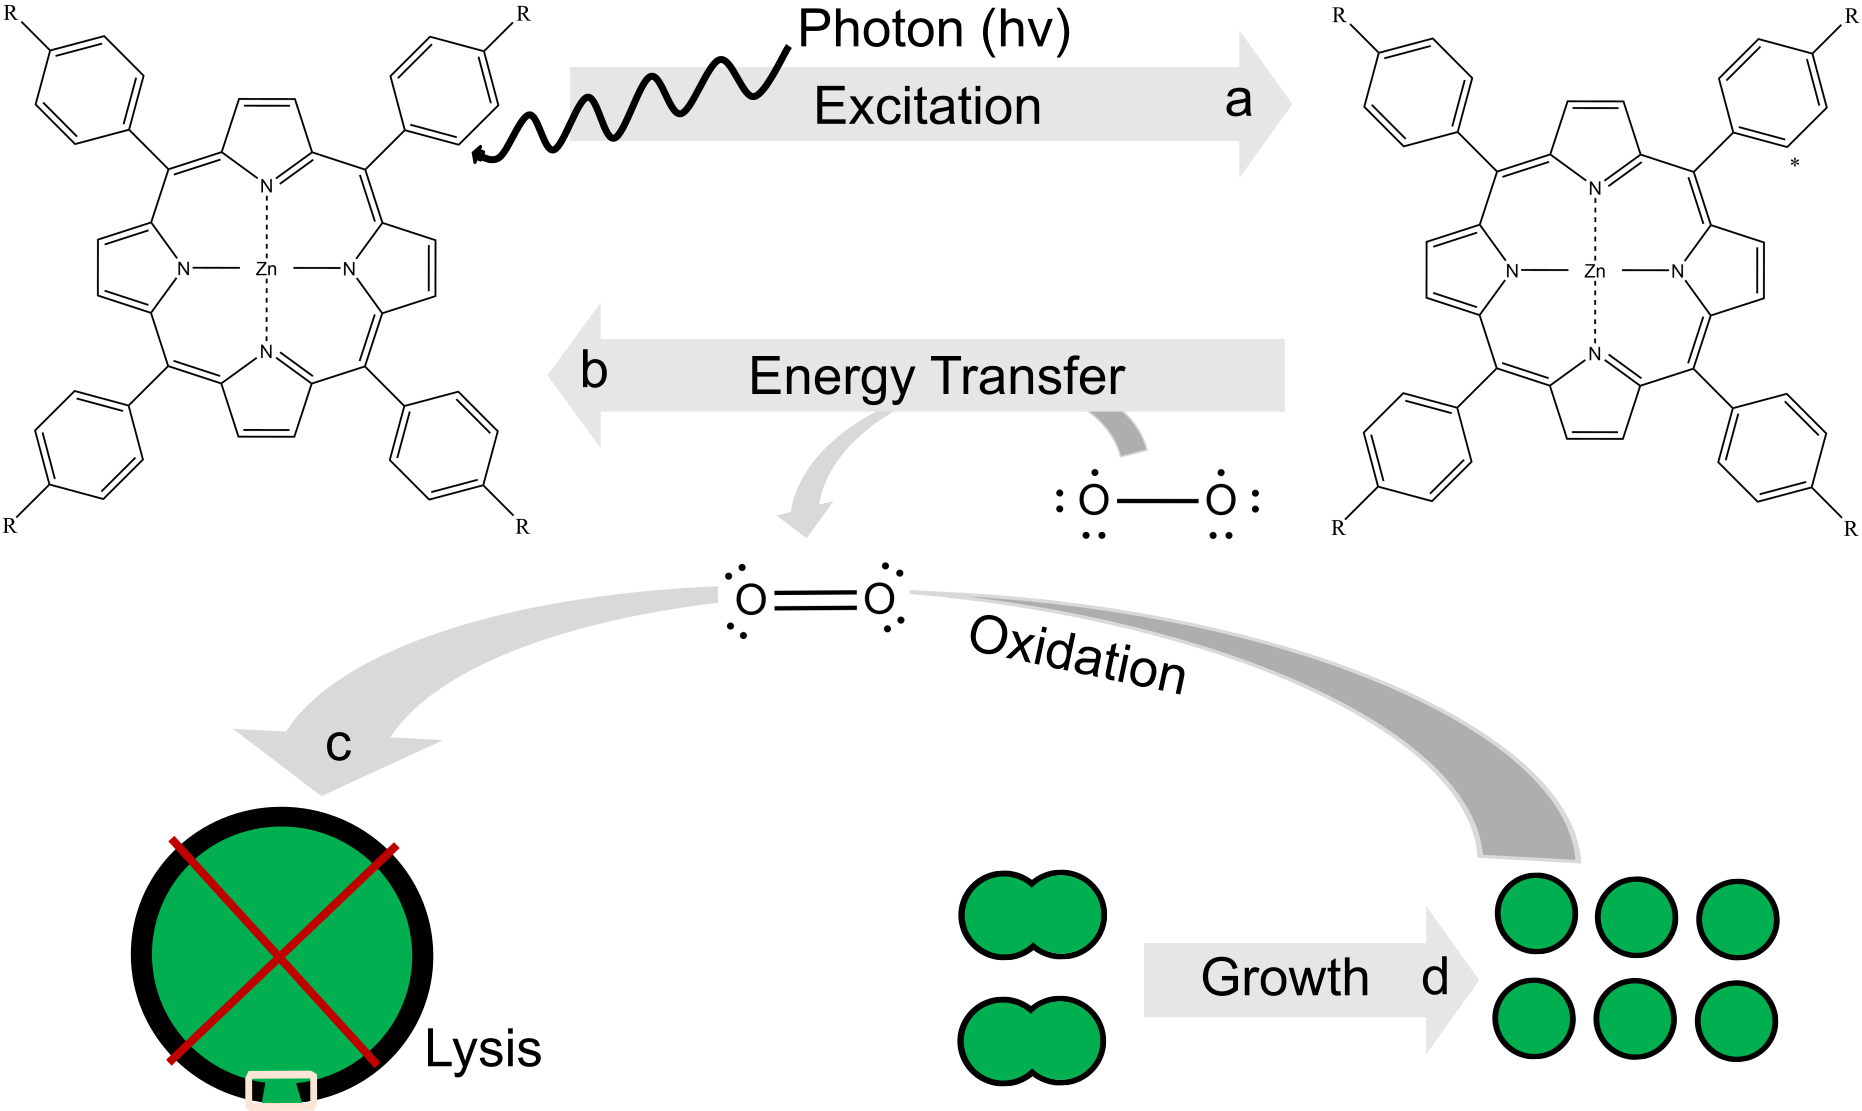
\includegraphics[width = \textwidth]{images/PDIpy/background/model.png}
    \caption{
        The conceptual model of PDI that is captured by our kinetic system. \textbf{Step a} is the  excitation of a photosensitizer (PS) via incident light at the wavelength to which the PS is tuned. \textbf{Step b} is the transfer of excitation energy from the excited PS to ambient oxygen, which reforms the PS catalyst and generates singlet oxygen. \textbf{Step c} is the oxidation of membrane phospholipids via singlet oxygen, which rapidly causes membrane lysis and subsequently cell death. \textbf{Step d} is the continuous growth of surviving organisms. Each of these processes are represented by chemical reactions and rate laws in our kinetic model.
    }
    \label{conceptual_model}
\end{figure}

\begin{figure}
    \centering
    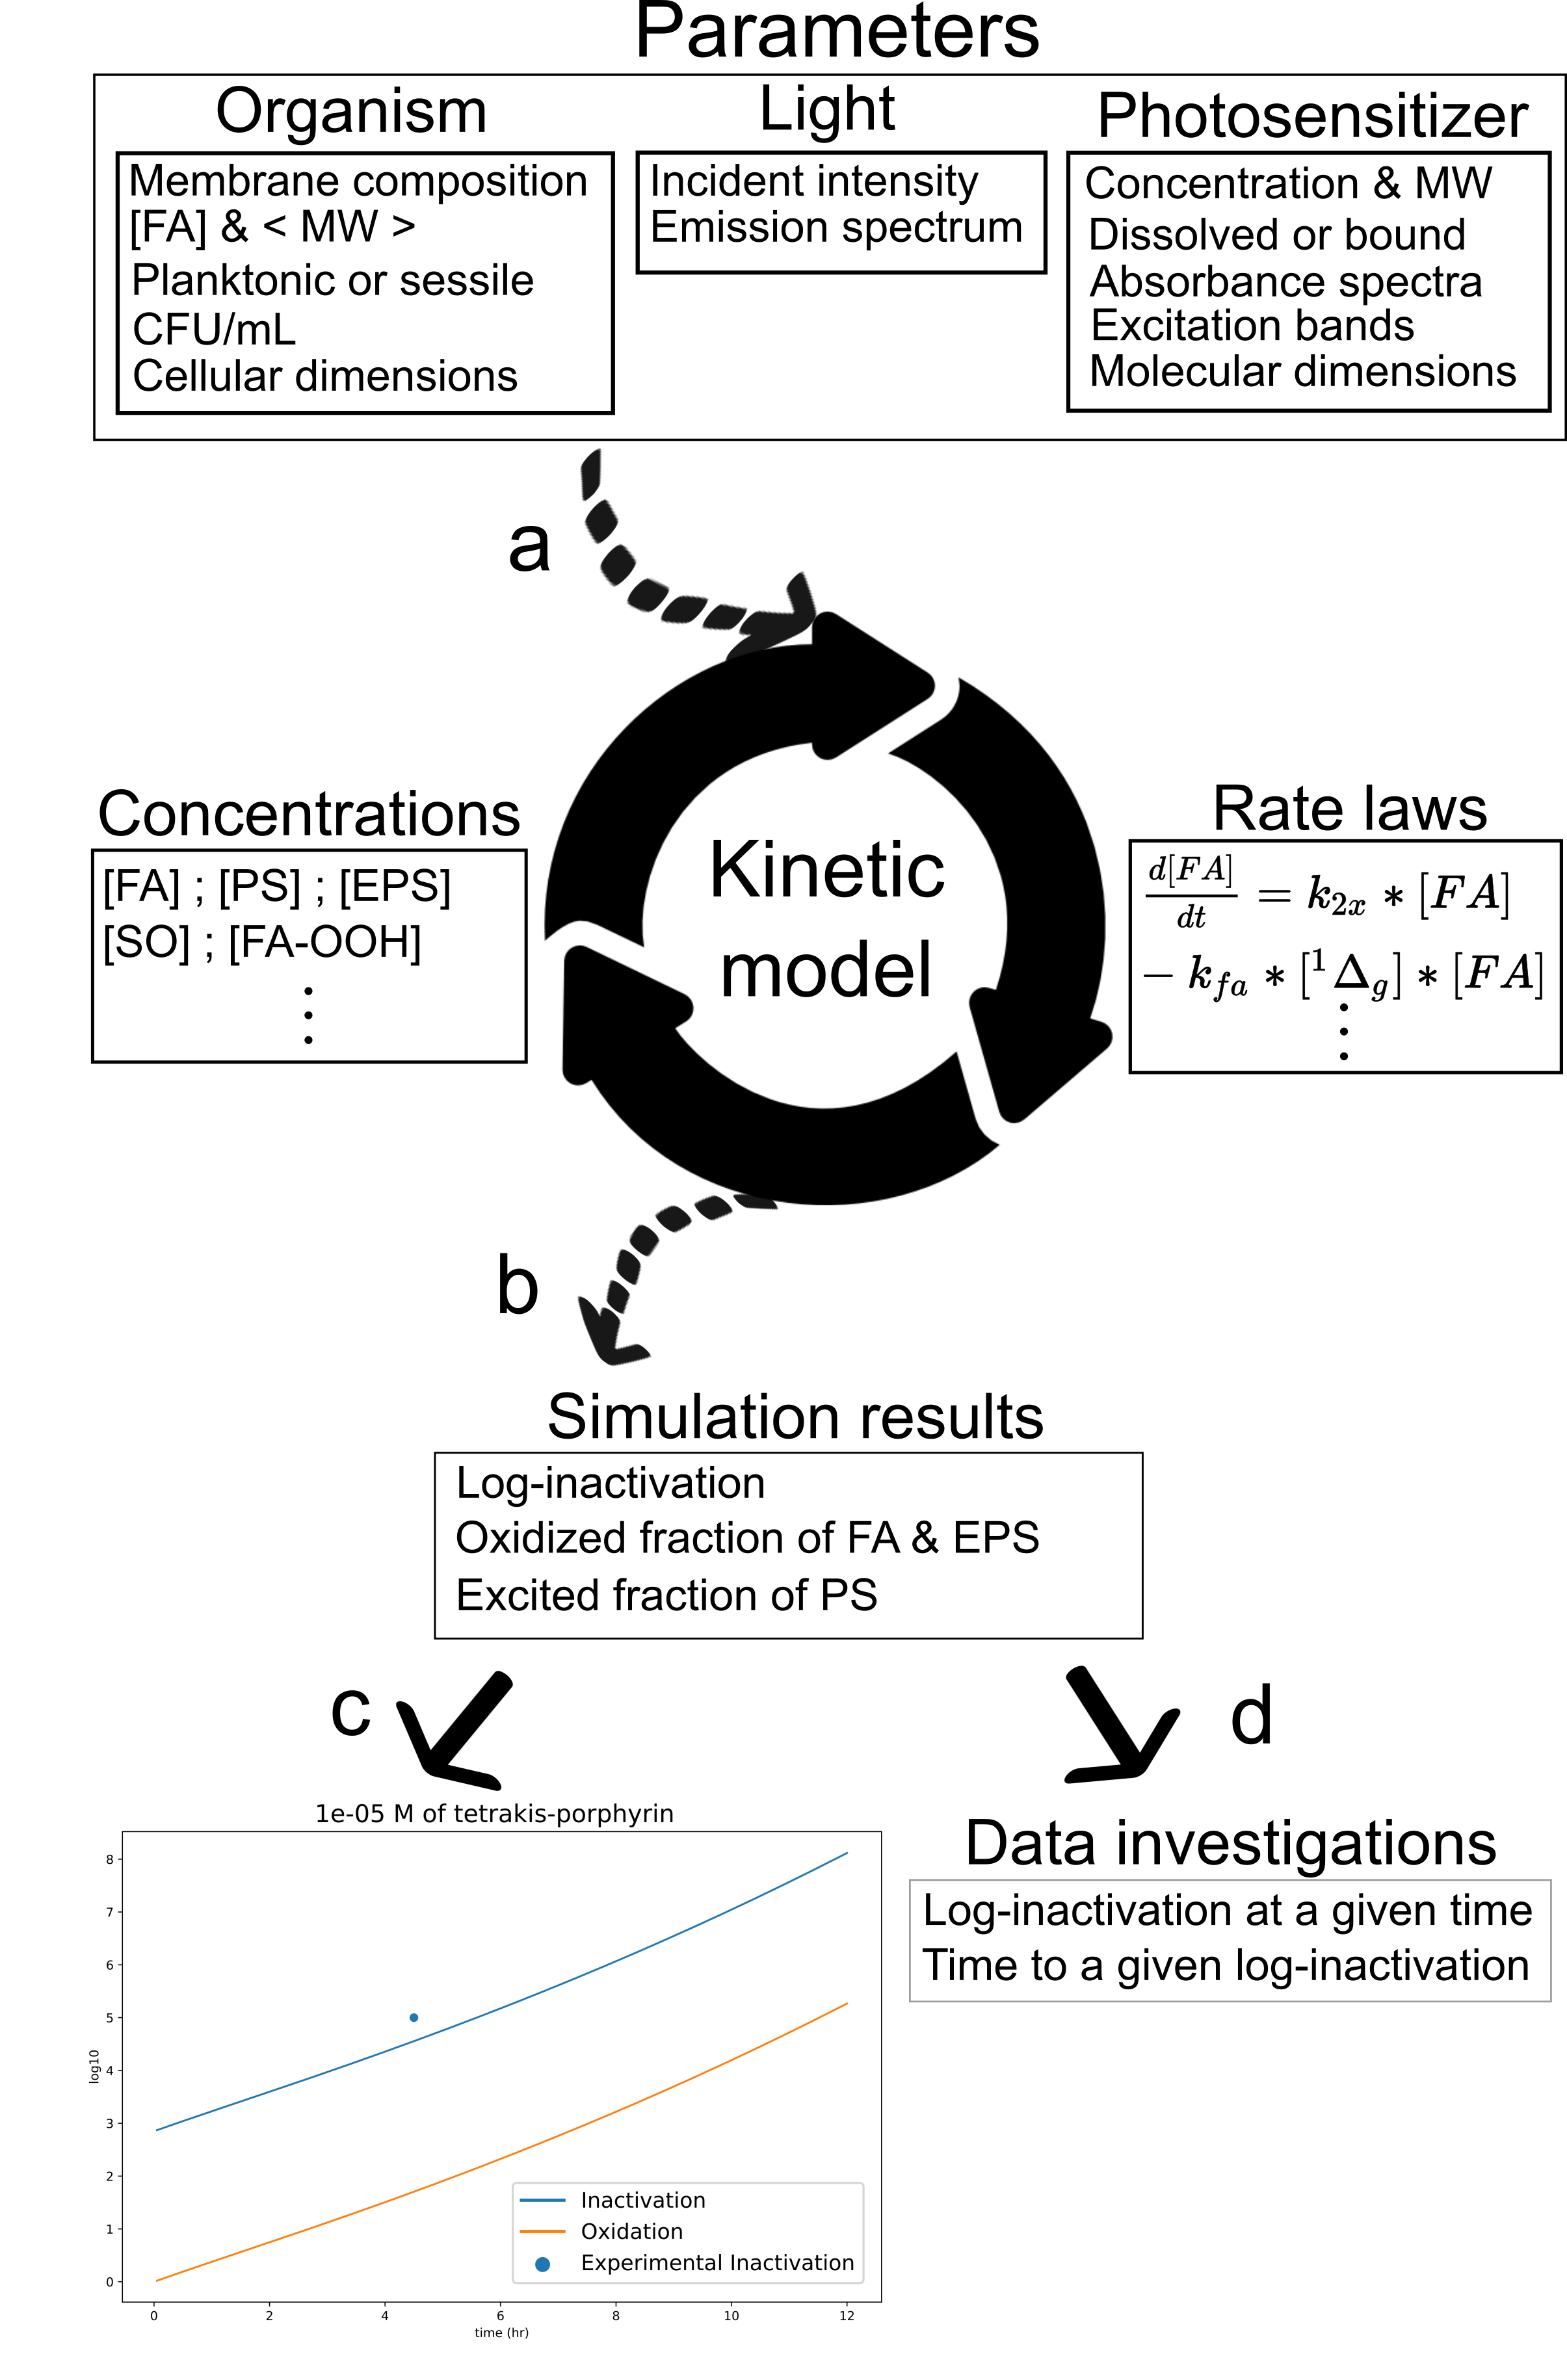
\includegraphics[width = 0.7\textwidth]{images/PDIpy/background/workflow_2.png}
    \caption{
        The programmatic workflow of PDIpy that implements our kinetic model. \textbf{Step a} describes the processing and substitution of simulation parameters -- categorically pertaining to the organism, light, and photosensitizer -- into the rate laws of our kinetic model. \textbf{Step b} executes the populated kinetic model through Tellurium, where concentration changes are calculated via rate laws and concentrations are updated with each timestep. The simulation yields predicted fractions of oxidized membrane fatty acids and excited PSs, which are converted into predictions of inactivation via a calibrated parameter. \textbf{Step c} graphically depicts the simulation results with the user-defined specifications. \textbf{Step d} investigates the two-dimensional data of predicted inactivation over time by slicing through either variable via a built-in function.
    }
    \label{workflow}
\end{figure}

\section{Methods} \label{methods}
\subsection*{Conceptual model}
Our model represents an experimental PDI system with i) a porphyrin PS, ii) a coccus (spheroid) bacteria such as \textit{S. aureus}, iii) a constant light source, and iv) an aqueous solution that contains a steady-state of dissolved oxygen. The bacteria are represented by fatty acid chains, which our model assumes is the cite of membrane oxidation and hence is the only pertinent bacterial aspect for extracellular PDI. Biofilms, for simulations of sessile systems, are represented as a combination of fatty acid chains (bacteria) and extracellular polymeric substances (EPS) in a predefined ratio for the simulated species, which our model assumes is the cite of oxidation in the biofilm matrix. The model calculates the interaction of $^1\Delta_g$ within the membrane volume or the volume of EPS, since this is the location of PDI inactivation.

Each aspect of this model is represented with a variable: i.e. the PS absorptivity (which can be approximated from molecular dimensions), and the $\frac{mol}{vol}$ or $\frac{mol}{area}$ concentration; the cellular state (planktonic or sessile), and the $\frac{CFU}{mL}$ for planktonic experiments; and kinetic constants for some PDI reactions. These variables are populated in $8$ chemical reactions that can be categorized into $4$ general processes: a) photoexcitation and photobleaching, $\ce{^1PS ->[h\nu] ^3PS}$ in \cref{ps_excitation_steps}; b) energy transfer, $\ce{^3PS ->[energy] ^3\Sigma_g^-}$ in \cref{excited_ps_steps}; c) the oxidation of biological substrates; and d) growth of the pathogen. A complete description of these reactions and their respective rate laws is represented in Table \ref{reactions_table}. Each reaction is each detailed in the following sub-sections.

\begin{table}
    \centering
    \begin{tabular}{c|c|c}
        \textbf{Name} & \textbf{Reaction} & \textbf{Rate law} \\
        \toprule
        Photoexcitation & \ce{^1PS <=>[k_{ex}][k_f] ^3PS} & $\frac{d[\ce{^3PS}]}{dt} = k_{ex} * \frac{photons_{PS}}{photons_{total}} * \Phi_{ex}*[\ce{^1PS}] - k_{f}*[\ce{^3PS}]$\\ \midrule
        Energy transfer & \ce{^3PS + ^3\Sigma_g^- -> ^1PS + ^1\Delta_g} & $\frac{d[^1\Delta_g]}{dt} = k_{transfer}*\Phi_{transfer}*[^3PS]*[^3\Sigma_g^-]$\\ \midrule
        Photobleaching & \ce{^1PS + ^1\Delta_g -> ^1PS_{bleached}} & $\frac{d[\ce{^1PS_{bleached}}]}{dt} = k_{bleaching} * [\ce{^1PS}]*[^1\Delta_g]$\\ \midrule
        Phosphorescence & \ce{^1\Delta_g -> ^3\Sigma_g^-} & $\frac{d[^3\Sigma_g^-]}{dt} = k_{phosphorescence}*[^1\Delta_g]$\\ \midrule
        Membrane oxidation & \ce{^1\Delta_g + FA -> FA-OOH} & $\frac{d[FA-OOH]}{dt} = k_{fa}*[^1\Delta_g]*[FA]$\\ \midrule
        EPS oxidation & \ce{^1\Delta_g + EPS -> EPS-OOH} & $\frac{d[EPS-OOH]}{dt} = k_{EPS_{oxidation}}*[^1\Delta_g]$\\ \midrule
        Reproduction & \ce{->FA} & $\frac{d[FA]}{dt} = k_{doubling}*[FA]$ \\ \bottomrule
    \end{tabular}
    \caption{
        All chemical reactions of the PDI kinetic model. These reactions are individually detailed in the Methods Section \ref{methods}.
    }
    \label{reactions_table}
\end{table}

\subsubsection{Photoelectric reactions}
\paragraph{PS excitation}
PDI begins with the excitation of the PS via an incident photon. This occurs as the combined result of a photon i) entering the aqueous solution, ii) striking a PS, and then iii) exciting an electron in that PS. This sequence is encapsulated by the kinetic expression
\begin{multline} \label{ps_excitation_kinetics}
    \frac{d[\ce{^3PS}]}{dt} =  k_{ex}*\frac{photons_{PS}}{photons_{total}} \\ 
    *\Phi_{ex}*[\ce{^1PS}] - k_{f}*[\ce{^3PS}]~. 
\end{multline}
The $k_{ex}$ \& $k_{f}$ rate constants are estimated as the inverse of the rise and decay times for the selected PS, respectively. The rise time for a porphyrin PS is approximated as $50 fs$ based upon estimates of $<100 fs$ \cite{Andersson1999PhotoinducedState} and $[60,90]~ fs$ in ethanol solvent \cite{Gurzadyan1998Time-resolvedZn-tetraphenylporphyrin} that elongates the lifetime of excited molecules relative to water. The decay time, from the S2 fluorescence \cite{Akimoto1999UltrafastPorphyrins}, and $\Phi_{ex}$ ($\frac{PS excited}{photon absorbed}$) are approximated for a porphyrin PS to be $1.5 ns$ and $\approx 0.7$ \cite{Krasnovsky2012PhotochemicalEnvironment}, respectively. The $\frac{photons_{PS}}{photons_{total}}$ \cite{Brasel2020AnAgalactiae}, which is the proportion of photons in the solution that strike a photosensitizer \cite{Santos2020ApplicationAureus}, can derive from either emission and absorption spectra of the incident light and the PS \cite{Gerola2012ChemicalPhotobleaching}, respectively, or the series of steps and approximations that are articulated in the Excitation Proportion section of the Supporting Information. The $[\ce{^1PS}]$ is finally provided in either molar or $\frac{mg}{area}$, where the latter unit for surface-bound PSs is converted into an effective molar of the PS in the volume within which the surface-bound PS resides immediately adjacent to the substratum surface. 

\paragraph{Photobleaching}
A PS may lose its absorptivity either by experiencing an irreversible rearrangement after collision with a photon -- which is described by an oxygen independent, first-order, reaction \cite{Bonnett1999PhotobleachingStudy,Mang1987PhotobleachingTherapy} -- or by being oxidized by $^1\Delta_g$ -- which is described by an oxygen dependent, second-order, reaction 
\begin{equation}
    \ce{^3PS + ^1\Delta_g ->[h\nu] PS-OOH}~.
\end{equation}
We developed a rate law 
\begin{equation} \label{bleaching_kinetics}
    \frac{d[\ce{^1PS_{bleached}}]}{dt} = k_{bleaching}*[\ce{^1PS}]*[^1\Delta_g]~,
\end{equation}
for our kinetic model that incorporates both the direct effects of $^1\Delta_g$ and the direct effects of light through $k_{bleaching} \approx 600 \frac{cm^2}{J*M}$ \cite{Dysart2005CalculationCells} which is a function of light exposure $\frac{W}{cm^2}$.

\subsubsection{Energy Transfer reactions}
The energy transfer $\ce{^3PS + ^3\Sigma_g^- -> ^1PS + ^1\Delta_g^}$ in \cref{excited_ps_steps} is described by the rate law
\begin{equation} \label{energy_transfer_kinetics}
    \frac{d[^1\Delta_g]}{dt} = k_{transfer}*\Phi_{transfer}*[^3PS]*[^3\Sigma_g^-]. 
\end{equation}
The rate constant $k_{transfer}$ is the inverse of the decay time of $\ce{^3PS}$, which for a porphyrin PS appears to be $100 ns$ in aqueous after accounting for the reported value \cite{Kupper2002KineticsOxygen} in acetone solvent which significantly increases the lifetime of excited states \cite{Spikes1992QuantumUroporphyrin}. The $^1\Delta_g$ phosphorescence side reaction, which often emits a specific infrared wavelength that can be measured to approximate the $[^1\Delta_g]$ \cite{Macpherson1993DirectCentres}, is kinetically represented 
\begin{equation}
    \frac{d[^3\Sigma_g^-]}{dt} = k_{phosphorescence}*[^1\Delta_g]
\end{equation}
where $k_{phosphorescence}$ is a function of $\frac{CFU}{mL}$, since the $^1\Delta_g$ lifetime is greater in biological material \cite{Maisch2007TheBacteria} than water \cite{Baier2005Time-resolvedCells}.

\subsubsection{Oxidation}
The following oxidation reactions consume oxygen, yet, our model assumes a steady-state of oxygen where the headspace of the simulated system perfectly replenishes consumed oxygen molecules.

\paragraph{Cytoplasmic membrane} 
The oxidation of cytoplasmic phospholipids, which we approximate as fatty acid (FA) chains, is represented as an irreversible reaction \cite{Watabe2007OxidationMembranes.}
\begin{equation} \label{membrane_oxidation}
    \ce{^1\Delta_g + FA -> FA-OOH}
\end{equation}
and a second-order rate law
\begin{equation} \label{membrane_oxidation_kinetics}
    \frac{d[FA-OOH]}{dt} = k_{fa}*[^1\Delta_g]*[FA]~.
\end{equation}
The rate constant $k_{fa} \approx 240 \frac{L}{g*s}$ \cite{Mukai2019KineticSolution} is reported with concentration in units of $\frac{g}{L}$, which we calculated from 1) the weighted average MW of the fatty acid chains in the cytoplasmic membrane, ii) the volume of the cytoplasmic membrane, and iii) an assumption that the cytoplasmic membrane volume consists entirely of fatty acid chains. 

\paragraph{Biofilm matrix} 
The oxidation of EPS, which represents the biofilm matrix, is reported to be significant during PDI \cite{Beirao2014PhotodynamicPorphyrin}. This process is represented through an irreversible reaction
\begin{equation} \label{EPS_oxidation}
    \ce{^1\Delta_g + EPS -> EPS-OOH},
\end{equation}
and a first-order reaction
\begin{equation} \label{EPS_oxidation_kinetics}
    \frac{d[EPS-OOH]}{dt} = k_{EPS_{oxidation}}*[^1\Delta_g]
\end{equation}
with an empirical rate constant of $37.75~\frac{1}{s}$ for \textit{S. aureus}, and an initial concentration of EPS that is $9x$ greater than the cellular mass \cite{Flemming2010TheMatrix}.
This reaction competes with \cref{membrane_oxidation} for $^1\Delta_g$ and thereby lessens the efficacy of PDI upon sessile organisms relative to planktonic organisms. 

\subsubsection{Microbial growth}
Cellular reproduction is simulated continuously as simply the increase in [FA] -- $\ce{->FA}$ -- since this is the only component of the cell that is pertinent to our model. The corresponding first-order rate law
\begin{equation}
    \frac{d[FA]}{dt} = k_{2x} * [FA]~,
\end{equation}
considers that growth is proportional with the current population of living microbes (represented by the fatty acids concentration). The rate constant $k_{2x}$ is the inverse of the doubling time of the simulated organism. 

\subsection{Inactivation fitting}

Inactivation is deduced from oxidation in our kinetic model by presuming an oxidative threshold for lysis around $0.01\%$ of the membrane fatty acids. This is implemented by geometrically translating the log10 predictions of oxidation, as a fraction of the total membrane fatty acids
\begin{equation} \label{oxidation_proportion}
    ox_{proportion} = \frac{[FA-OOH]}{[FA-OOH]+[FA]}~,
\end{equation}
by $\approx 4$-log: e.g. oxidation predictions of [3,4,5] become inactivation predictions of [7,8,9]. 

\begin{table}
    \centering
    \begin{tabular}{l|c|c}
        \textbf{Bacterial state} & \textbf{Hill parameter} & \textbf{Adjustment} \\
        \multirow{2}{0}{Planktonic} & EC50 & -76\% \\
         & nH & +100\% \\
         \midrule
         \multirow{2}{0}{Biofilm} & EC50 & -65\% \\
         & nH & +120\% \\
    \end{tabular}
    \caption{
        The Hill parameters adjustments that are enacted to create the inactivation plot for both planktonic and biofilm systems. 
    }
    \label{hill_parameters}
\end{table}

\subsection{Implementation}
The model was implemented in SBML \cite{Keating2020Models} through the Antimony syntax of the Tellurium Python module \cite{Choi2018Tellurium:Biology}. This standard model format was combined with a SED-ML description of the model figure \cite{Waltemath2011ReproducibleLanguage} into a COMBINE OMEX file \cite{Bergmann2014COMBINEProject}, which is transparent and reproducible representation of each simulation. 
\subsubsection*{Model calibration}
The SBML model format may further enable the programmatic calibration of the lysis threshold parameter through training data and the COPASI software \cite{Bergmann2017COPASIBiotechnology}. This lysis threshold is not reported in literature; hence, this threshold, which emerges from our model, is an original prediction and typifies the value of a mechanistic model that can elucidate opaque details.

\paragraph{Beirao et al.}
The Beirao et al. study \cite{Beirao2014PhotodynamicPorphyrin}, which examined the efficacy of a dissolved PS over a range of concentrations against both planktonic and sessile states of \textit{S. aureus}, was used as a training data set. The training procedure included: a) recreating each reported trial through our model, and b) empirically adjusting the threshold parameter such that the total variance across all of the trials is minimized. The final \%-errors between the calibrated predictions and the reported values from each trial are depicted in Table \ref{beirao_et_al_data} and Figure \ref{beirao_et_al}. 

\begin{table}
    \centering
    \begin{tabular}{c|c|c|c|c|c}
        Bacterial & [PS] & Inactivation & Reported & Predicted & \multirow{2}{1.2cm}{\%-error}\\
        state & ($\mu M$) & (-log10) & (min) & (min) & \\
        \toprule
        \multirow{3}{1.5cm}{planktonic} & 5 & 7.6 & 51 & 87 & 60\\
        & 10 & 7.6 & 51 & 39 & -23\\
        & 20 & 7.6 & 30 & 18 & -40\\
        \midrule
        \multirow{3}{1.5cm}{sessile} & 5 & 3.6 & 270 & 247 & -9\\
        & 10 & 5 & 270 & 337 & 25\\
        & 20 & 6.3 & 270 & 256 & -5\\
        \bottomrule
    \end{tabular}
    \caption{
        A quantitative comparison of inactivation data from Beirao et al. versus PDIpy predictions after its calibration. 
    }
    \label{beirao_et_al_data}
\end{table}

\begin{figure}
    \centering
    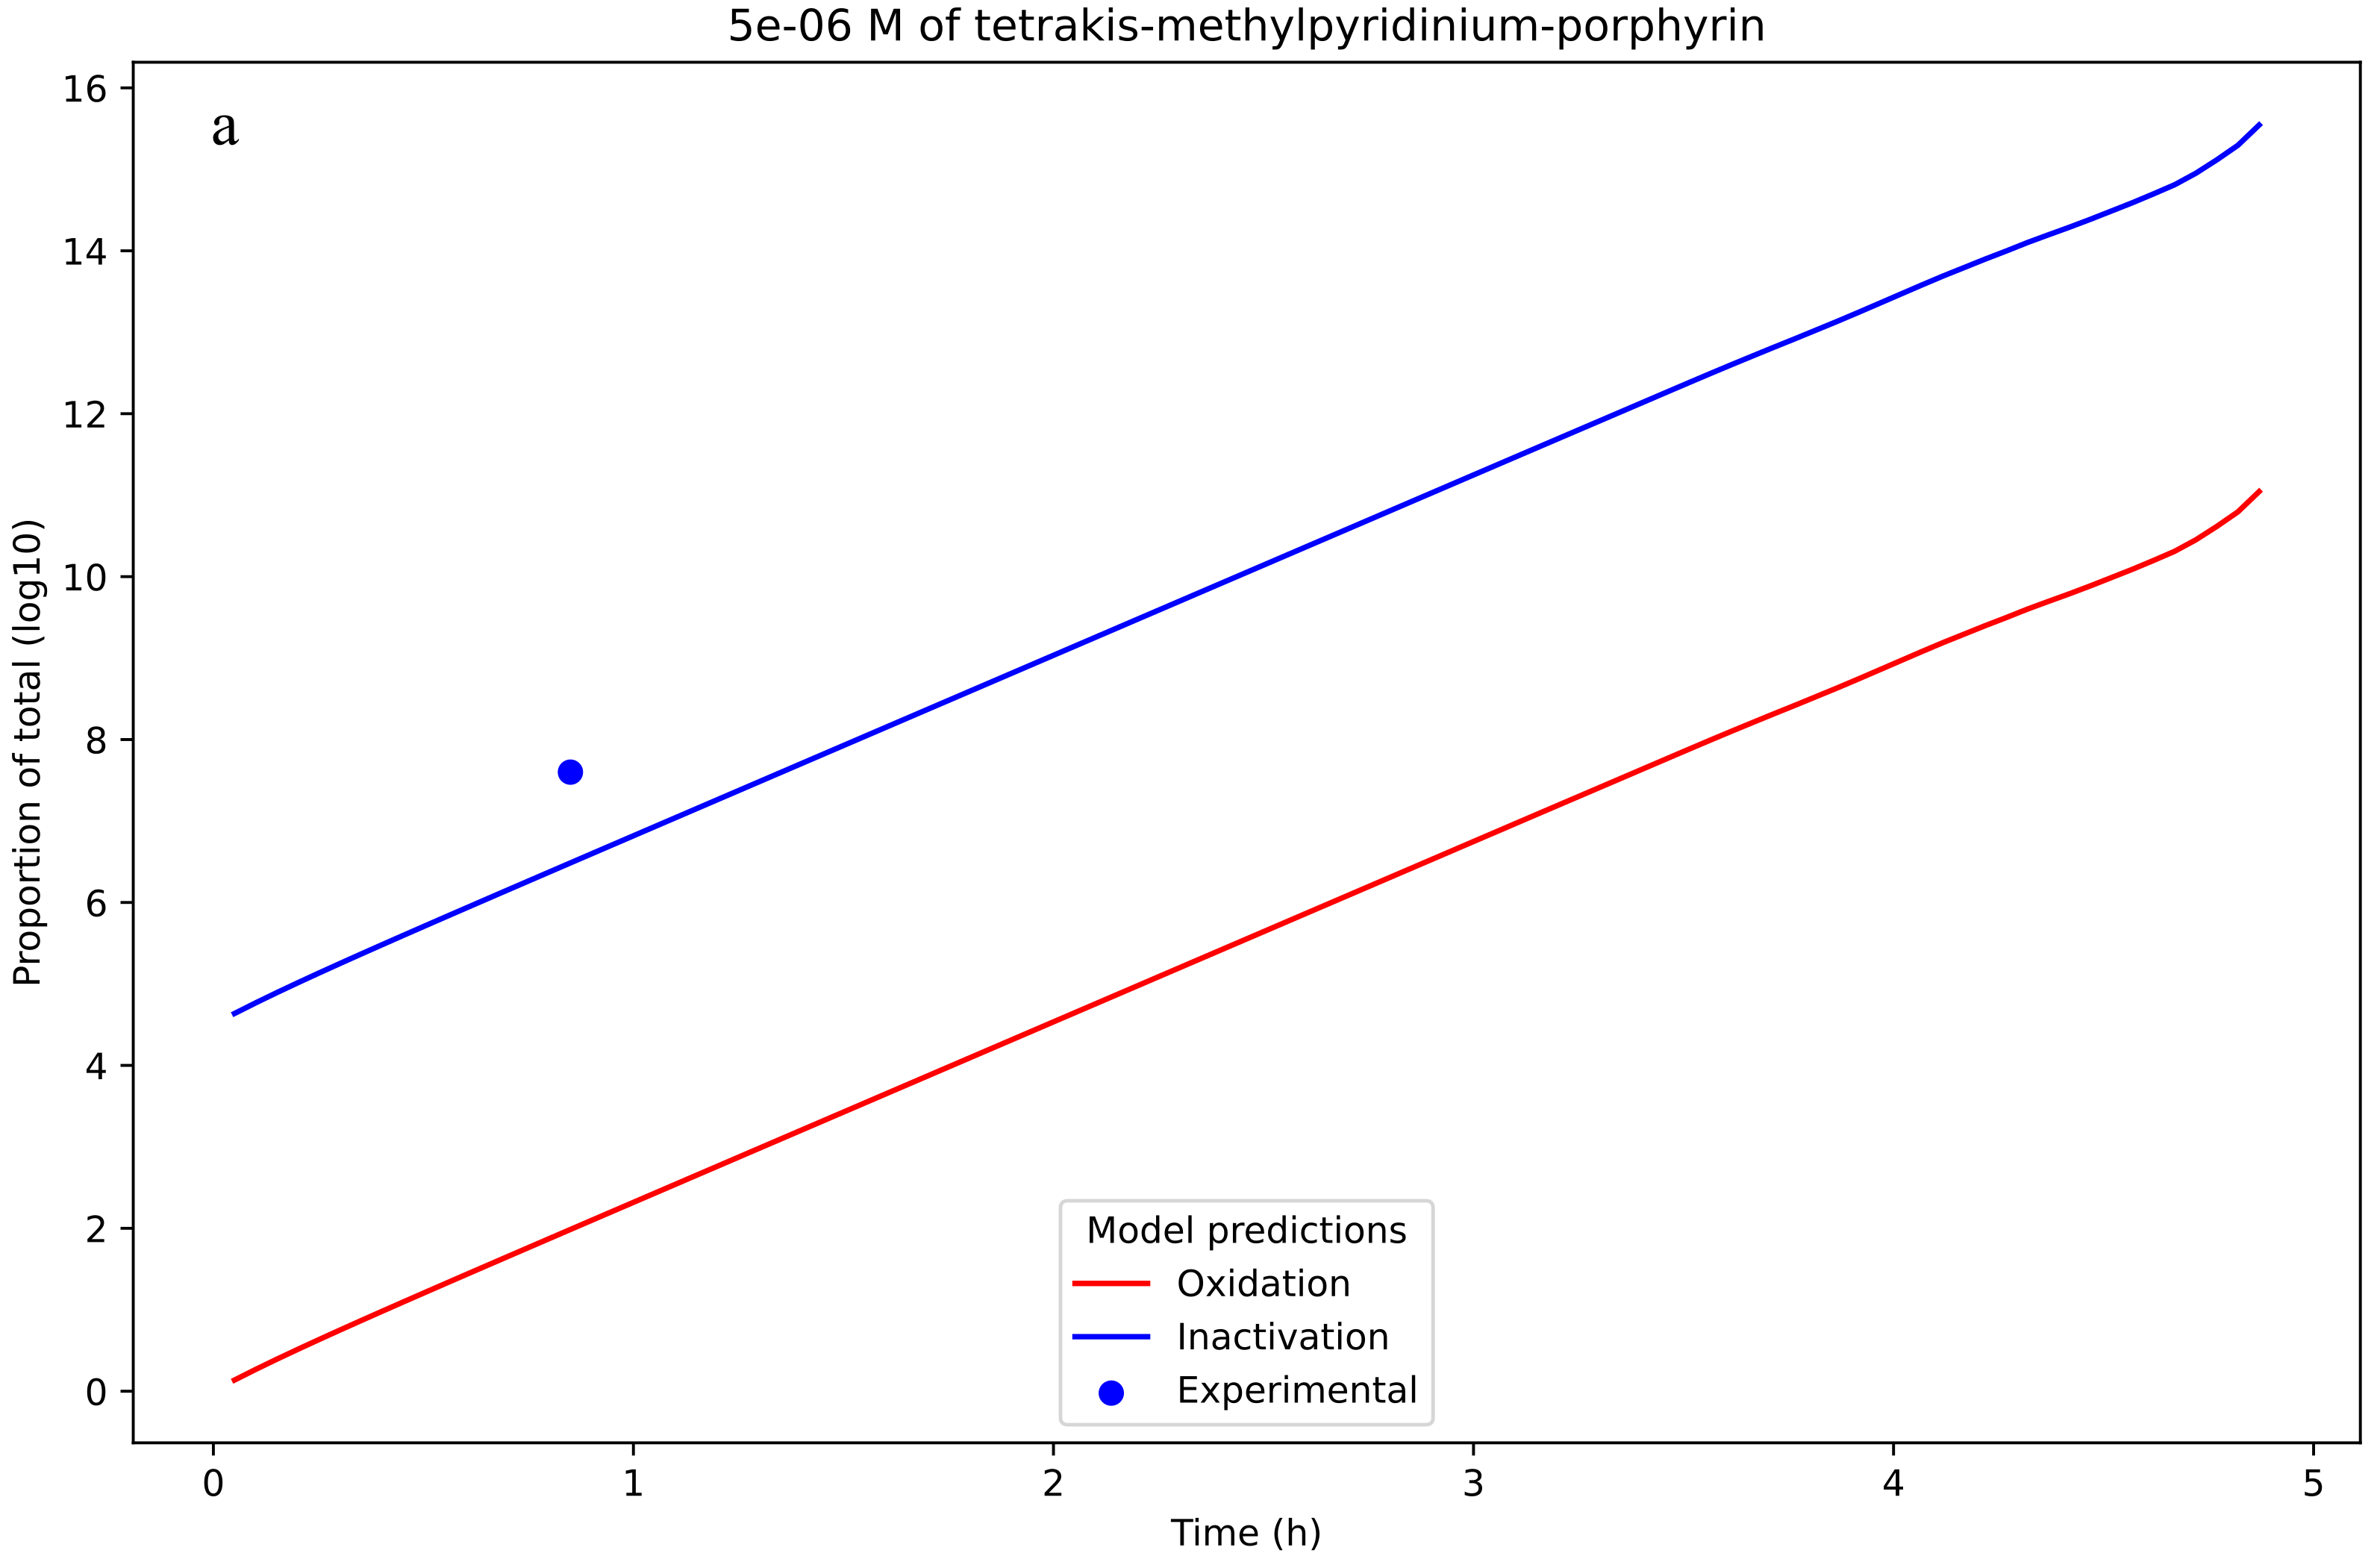
\includegraphics[width = 0.9\textwidth]{images/PDIpy/training/5uM.png}
    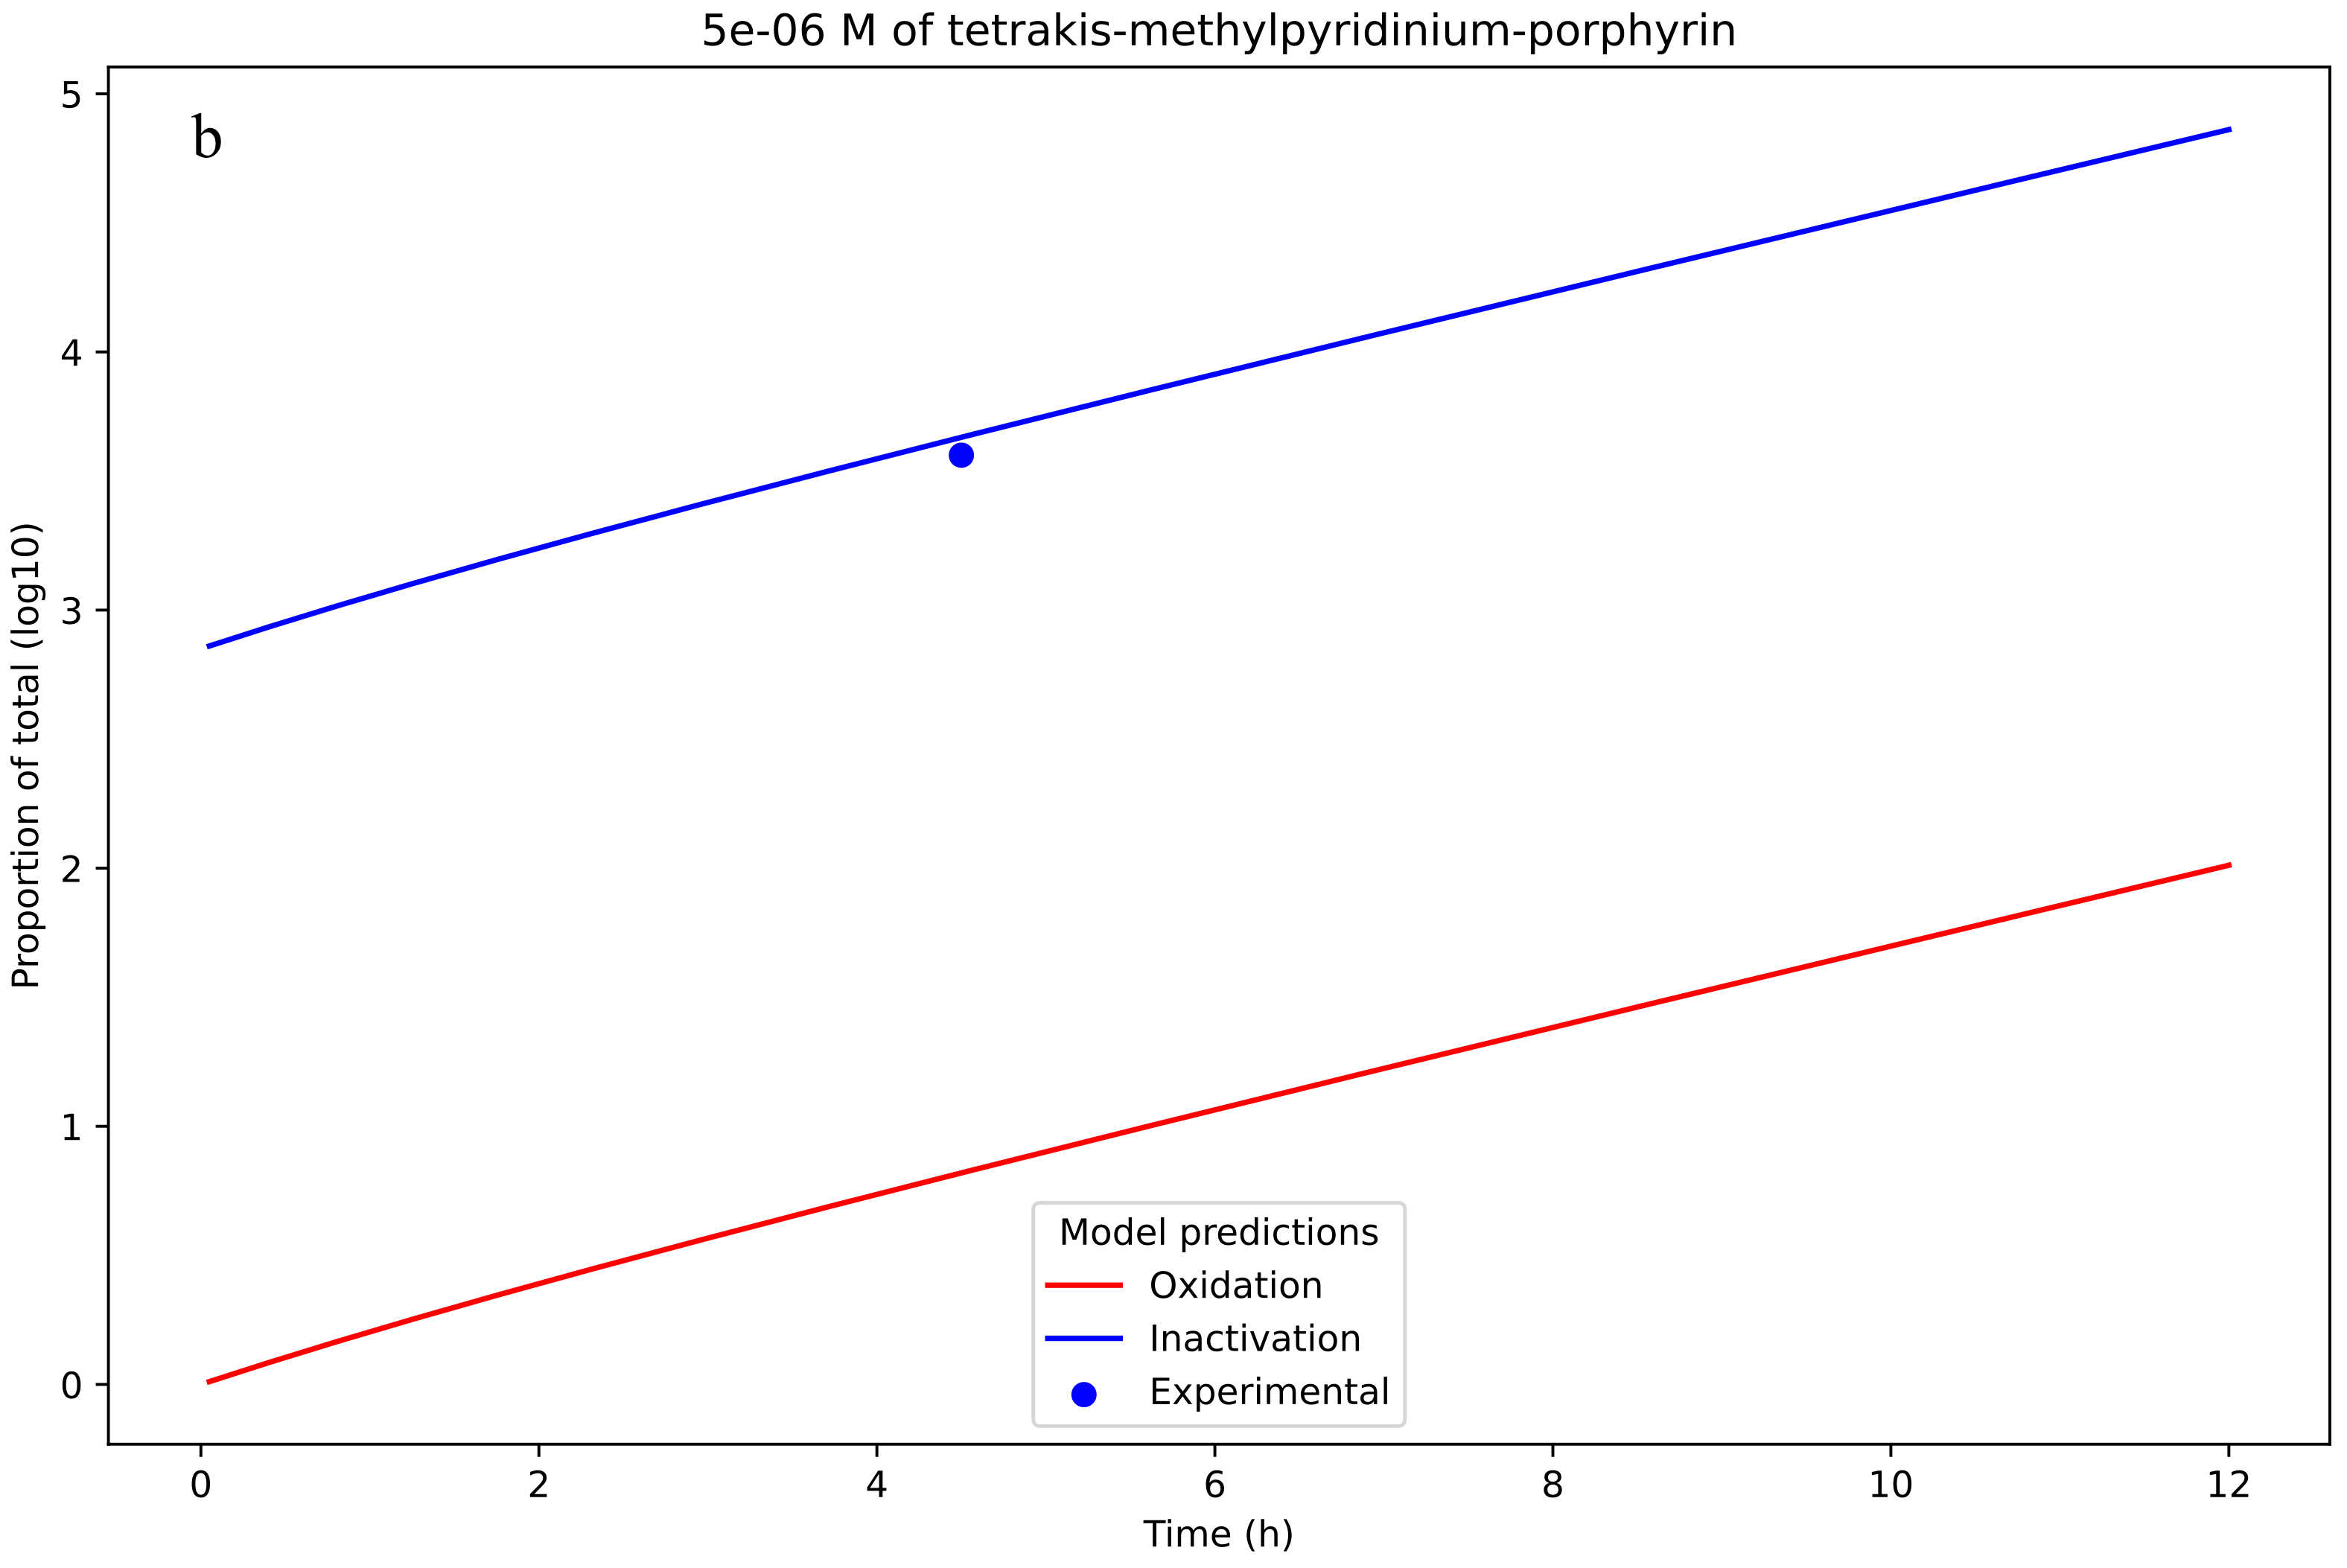
\includegraphics[width = 0.9\textwidth]{images/PDIpy/training/5uM_biofilm.png}
    \caption{
        Model predictions of the Beirao et al. training data for a) planktonic and b) sessile states, where the dot signifies the reported datum from the trial experiment.
    }
    \label{beirao_et_al}
\end{figure}

\section*{Sensitivity analyses}

Numerous sensitivity analyses were conducted to determine the significance of experimental variables for PDI efficacy, which can signal worthwhile variables for further experimentation. One of these analyses is highlighted in the following section, while the other analyses are detailed in the Supporting Information. 

\paragraph{Light intensity}
The sensitivity of PDI inactivation to light intensities was explored across a 4-log range of $Lux$ values. The trend over this range, which is represented by Figure \ref{light_intensities}, reveals that the proportion of excited PS plateaus beyond $\approx 13,000~lux$. Direct inactivation from light, perhaps by exciting endogenous photosensitizers within cells \cite{Lippincott-schwartz2003PhotobleachingTechniques,Jin1995PhotolysisSolution,Itoh2001PhotodynamicPatients}, may still proportionally increase inactivation with light intensity beyond $\approx 13,000~lux$, however, these processes are currently not captured by our model. 

\begin{figure}
    \centering
    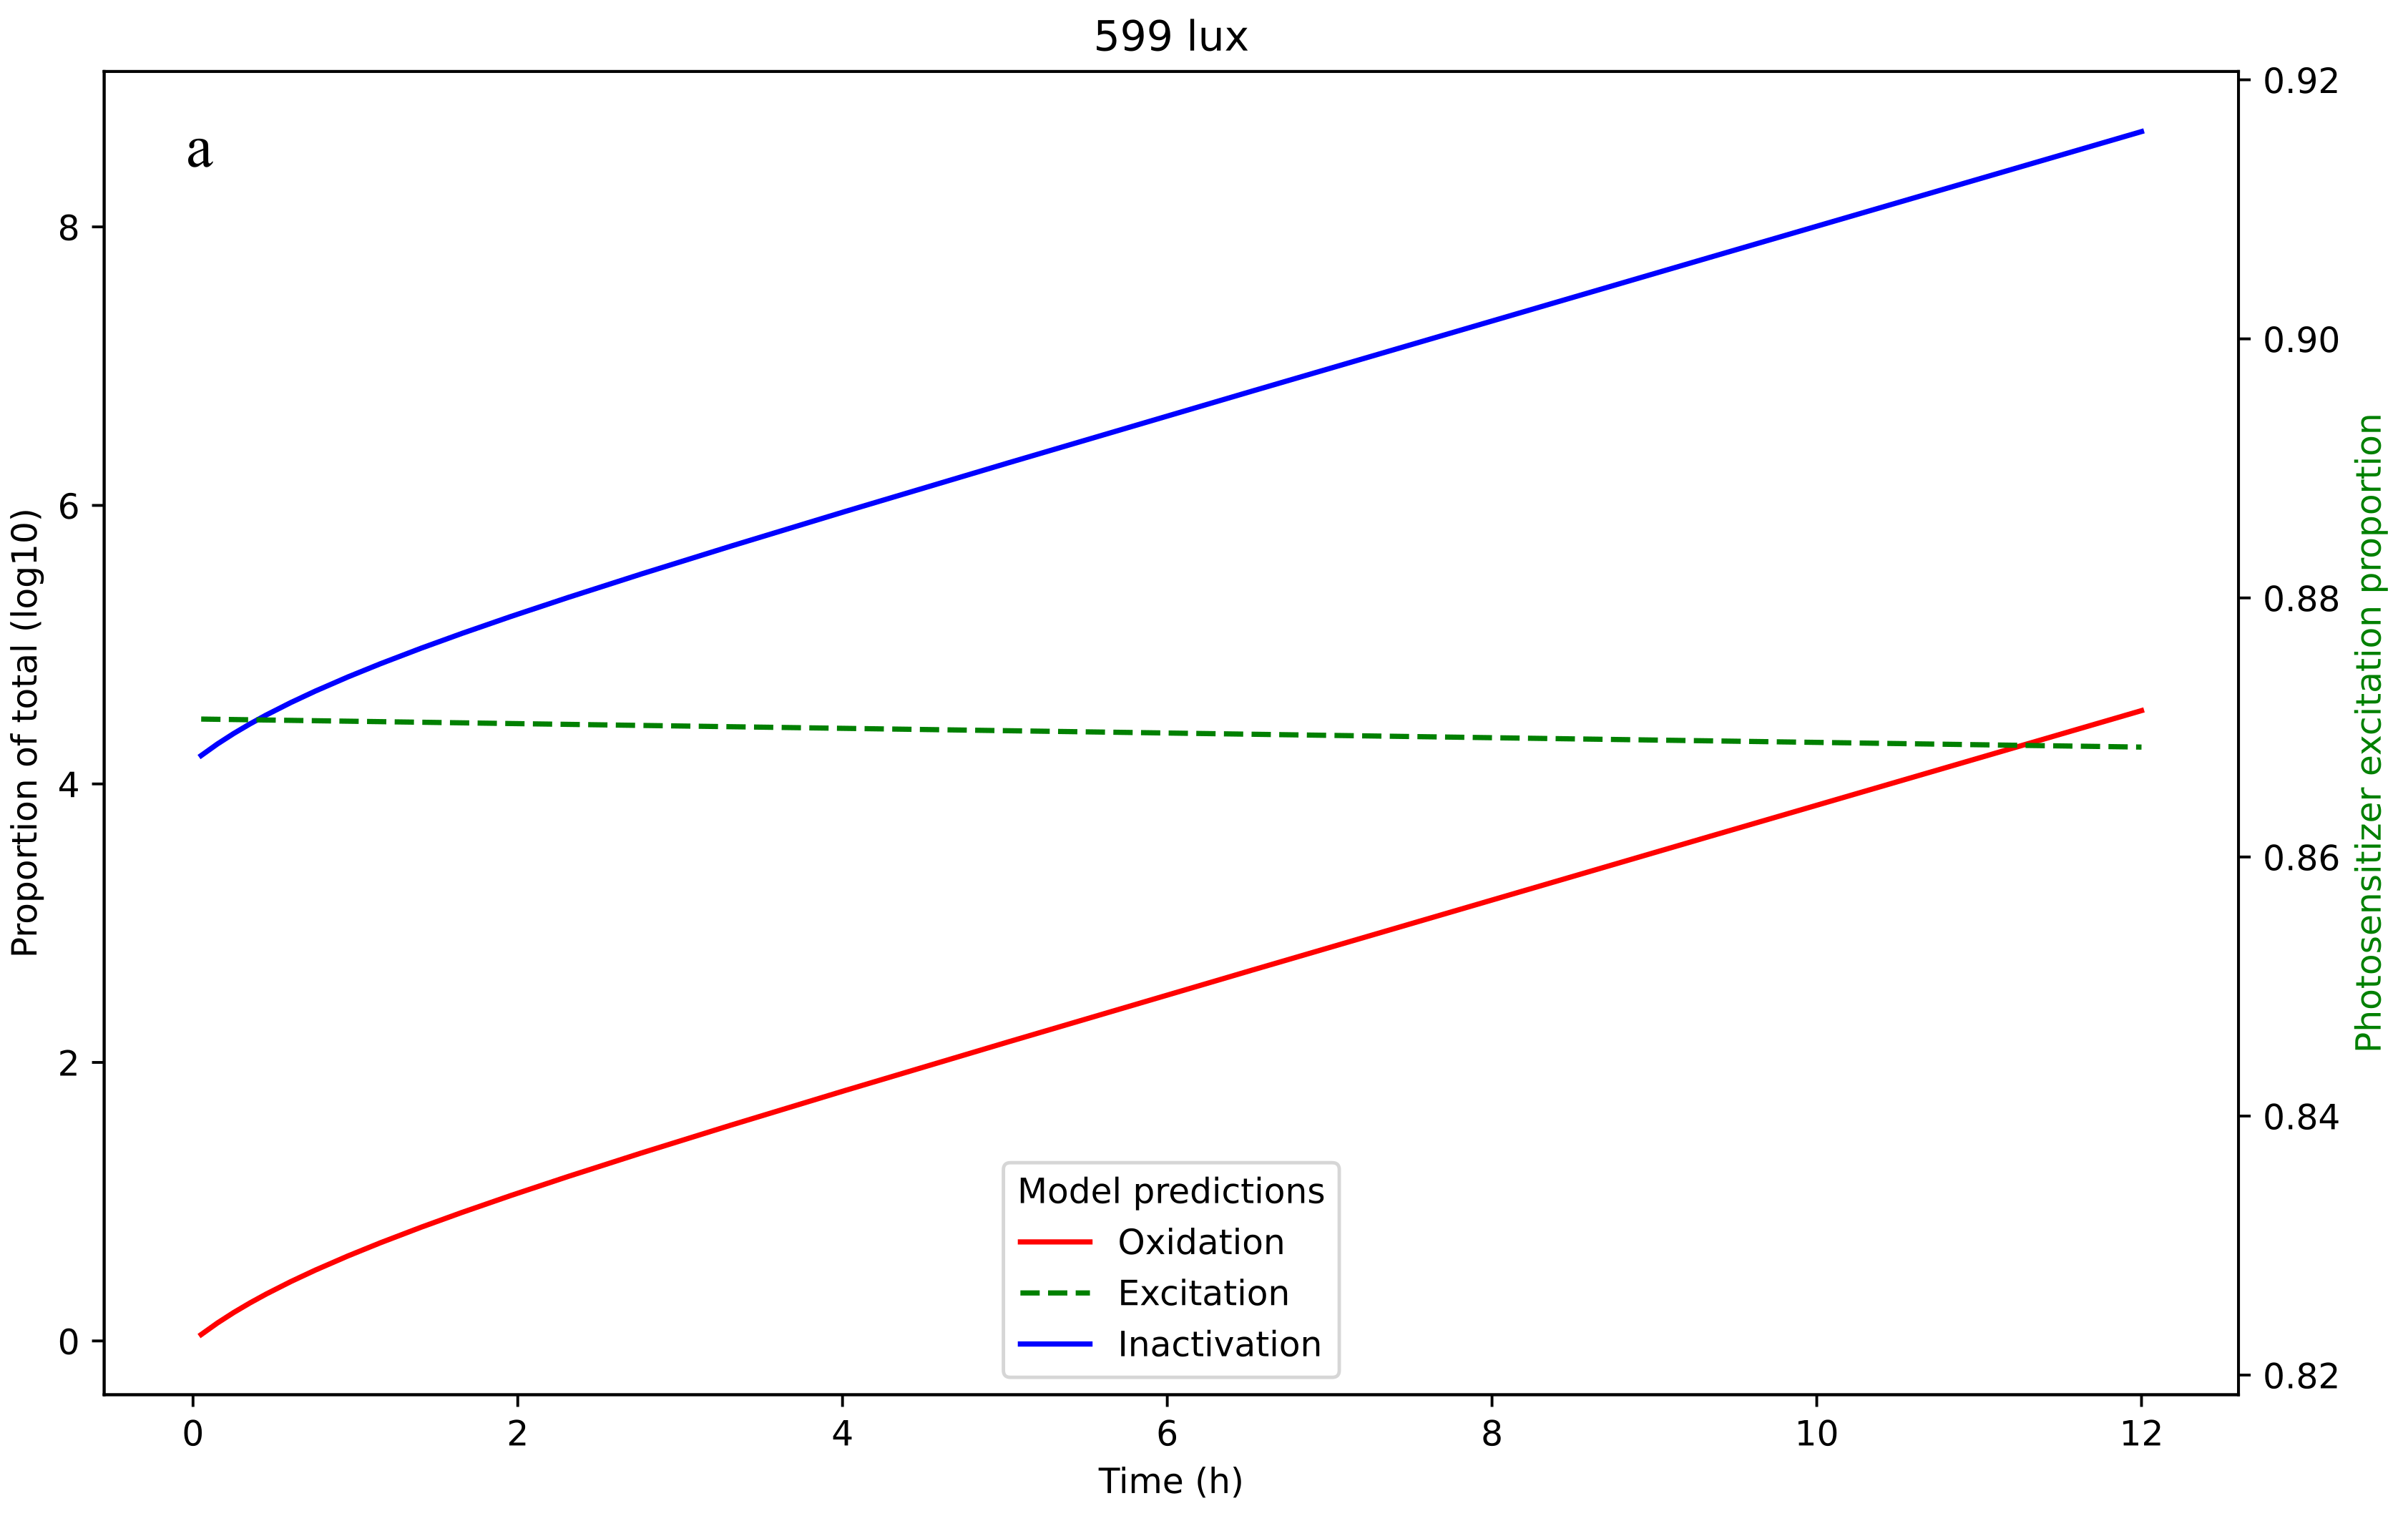
\includegraphics[width = 0.9\textwidth]{images/PDIpy/sensitivity_analyses/light_intensity/599_lux.png} \\
    \vspace{5mm}
    \midrule
    \vspace{5mm}
    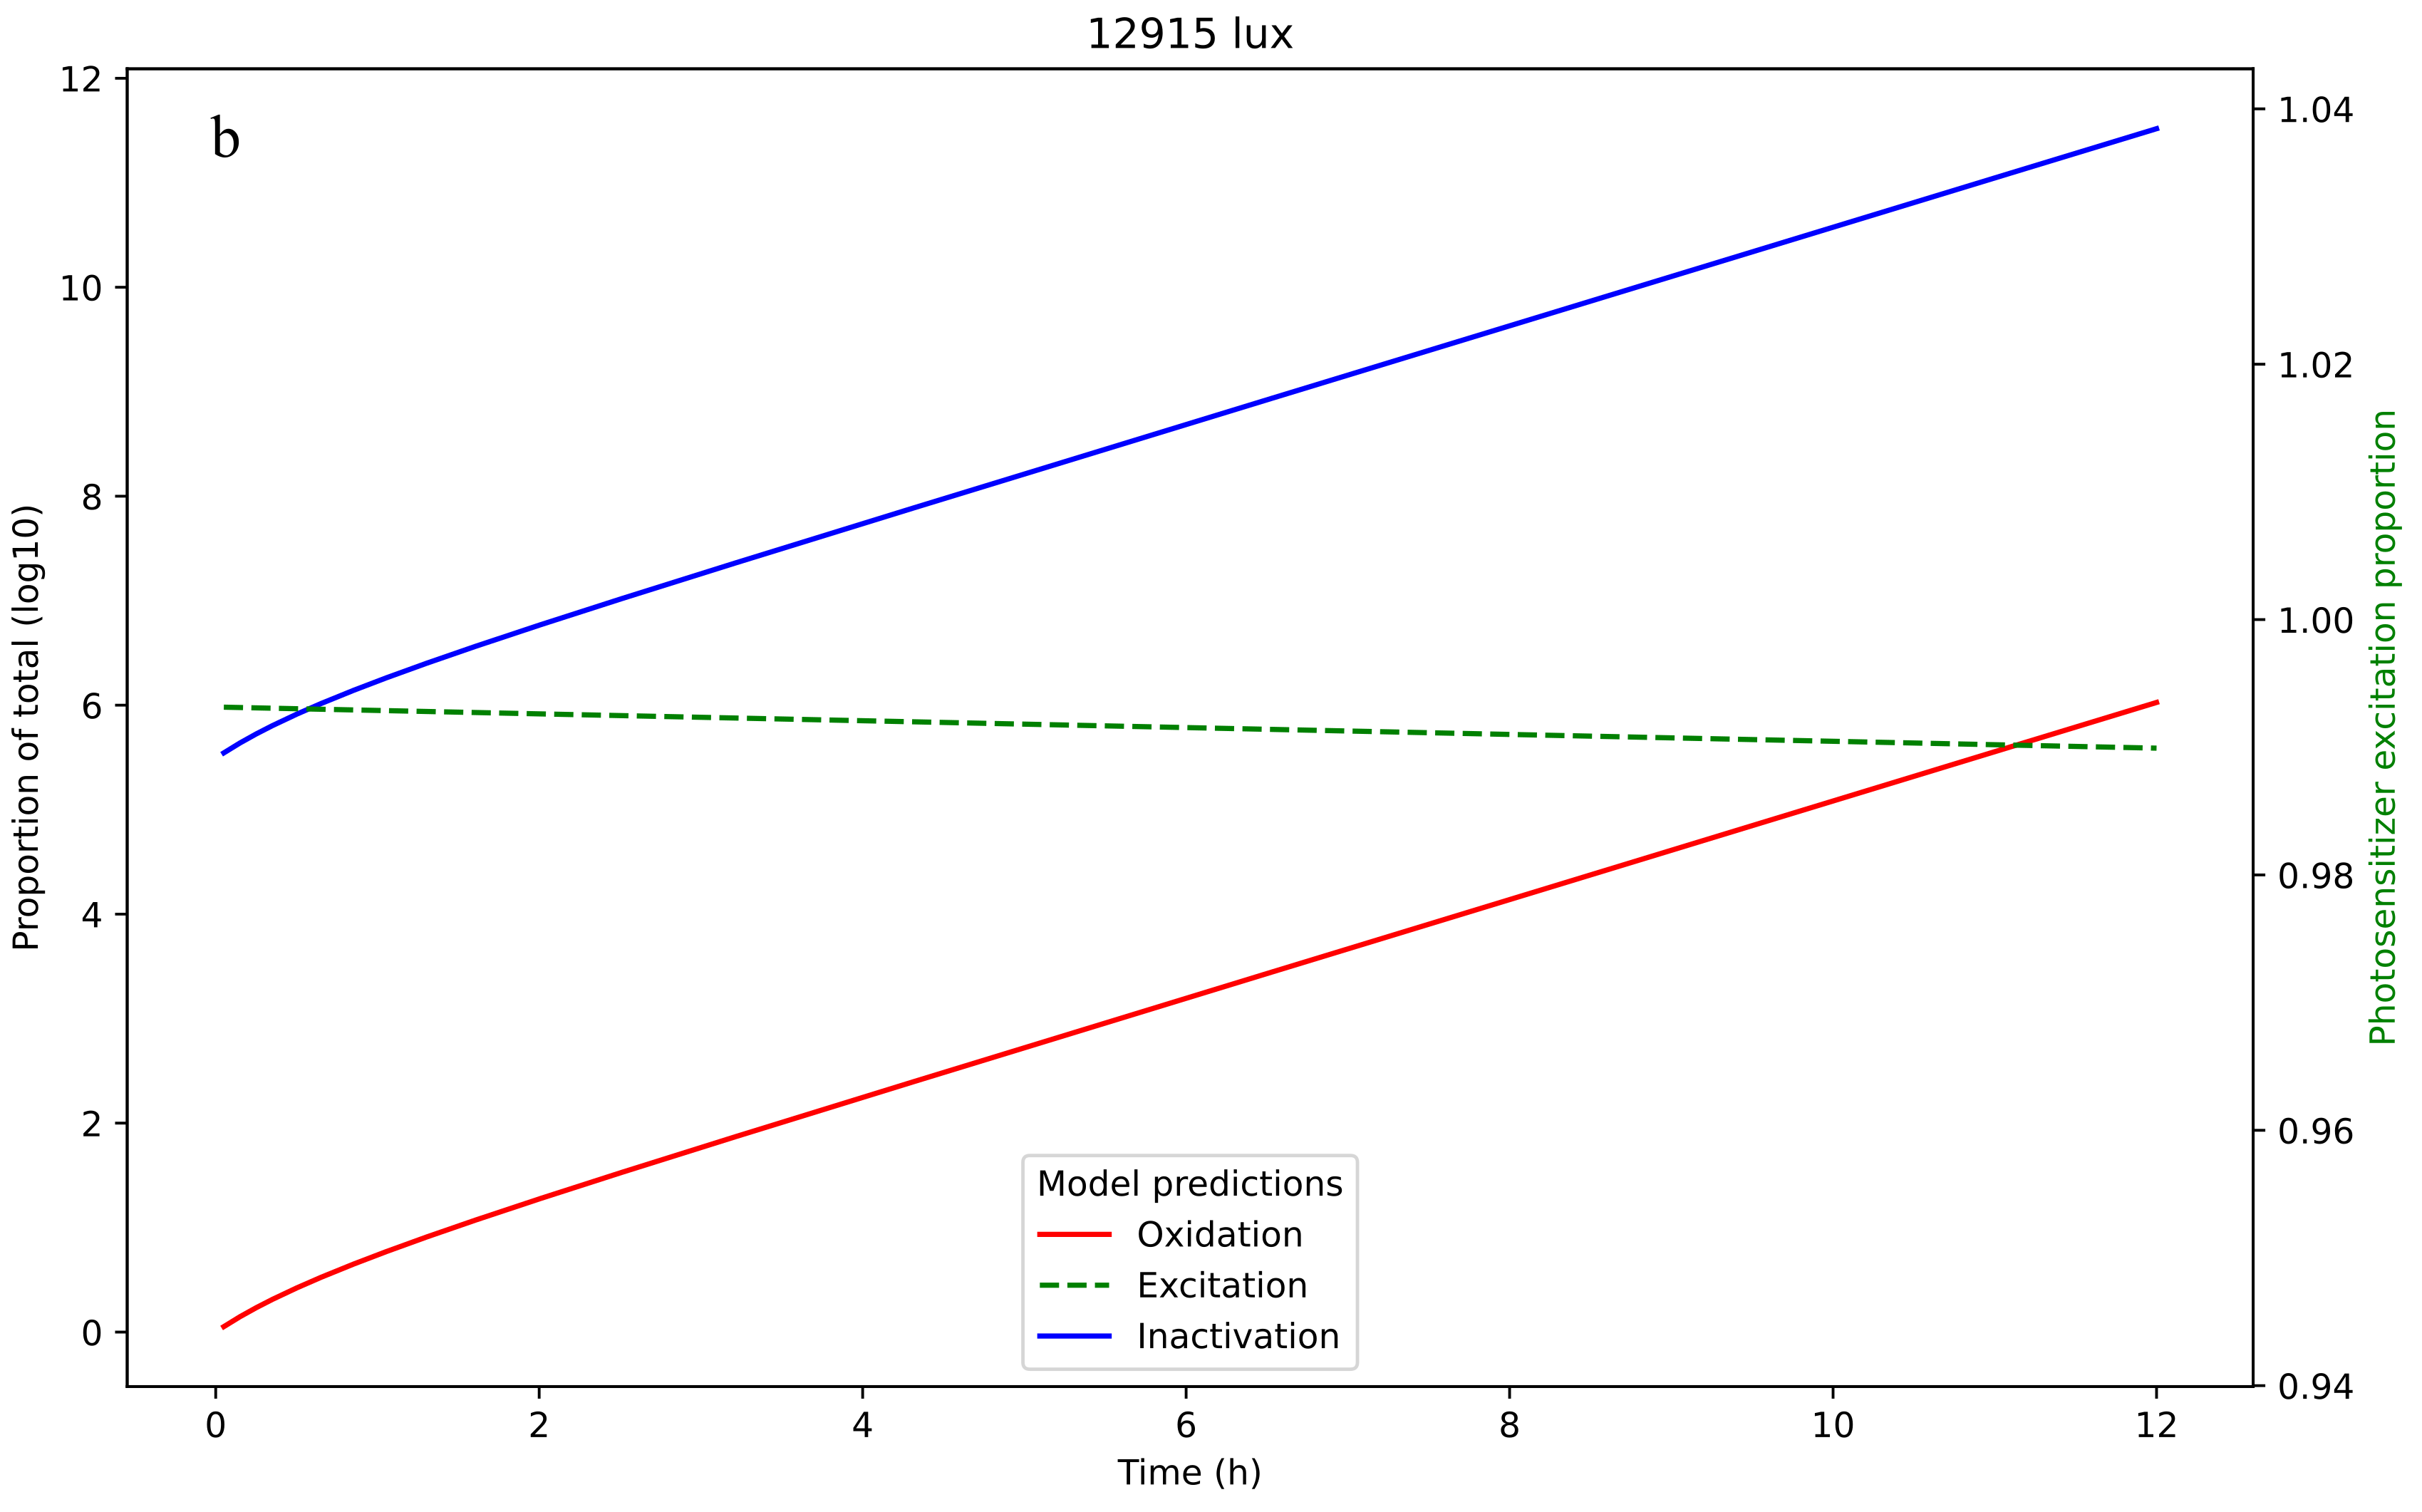
\includegraphics[width = 0.9\textwidth]{images/PDIpy/sensitivity_analyses/light_intensity/12915_lux.png}
    \caption{
        The proportion of excited PS, with the associated oxidation and inactivation predictions, at two contrasting light intensities: a) $599~Lux$, which approximates ambient indoor light, and b) $12915~Lux$, which approximates ambient daylight. The subtle negative slope that is proportion to the light intensity is the consequence of photobleaching, where incident photons can trigger irreversible rearrangements of the PS and thereby decrease the quantity of photoactive PSs over time.
    }
    \label{light_intensities}
\end{figure}

\\section*{PDIpy}
The kinetic model is defined as a Python API and is offered through the Python Package Index. Parameter files are also provided with default values for each category of the model variables, which provide an efficient and transparent means of parameterizing a simulation and which further supplement user-defined parameters. The complete list of accepted parameters and formats are detailed in the API documentation.

\section*{Discussion}
The alignment of model predictions and reported inactivations from our training set supports that the API and underlying kinetic model may guide the design of experimental PDI systems. The \%-error between the PDIpy predictions and the training data was interestingly greater in simulations of planktonic bacteria relative to sessile bacteria, which suggests that complexities of the planktonic phase -- e.g. PS permeability, which causes cytosolic oxidation -- are currently not captured by our kinetic model. 

The sensitivity analyses of the model variables illuminate its dynamic capacity to explore the space of PDI systems. This exhibits distinguishing features of this model, relative to other PDI models, to i) simulate diverse sets of experimental PDI conditions; ii) intuitively execute the kinetic model, and automatically visualize results, through the API interface; and iii) resolve the fundamental kinetics of PDI. We believe that this kinetic model and its open-source implementation as PDIpy will support developing PDI applications that can confront the looming crisis of AMR.

\section{Author Contributions}
\begin{description}
    \item[APF] Designed, executed, and codified the project.
    \item[JRK] Guidance and manuscript edits.
    \item[HLB] Guidance, manuscript edits, and funding.
\end{description}

\section{Acknowledgments}
The authors are grateful to Ethan Sean Chan for developing the framework of iPDIpy, which will be introduced in a future release of PDIpy. The authors thank the members of the Buckley and Wolff Groups at the University of Victoria for contributing ideas and data that were used to refine this PDI model. 